%!TEX TS-program = xelatex
\documentclass[11pt]{article}

\usepackage[english]{babel}

\usepackage{amsmath,amssymb,amsfonts}
\usepackage[utf8]{inputenc}
\usepackage[T1]{fontenc}
\usepackage{stix2}
\usepackage[scaled]{helvet}
\usepackage[scaled]{inconsolata}

\usepackage{lastpage}

\usepackage{setspace}

\usepackage{ccicons}

\usepackage[hang,flushmargin]{footmisc}

\usepackage{geometry}

\setlength{\parindent}{0pt}
\setlength{\parskip}{6pt plus 2pt minus 1pt}

\usepackage{fancyhdr}
\renewcommand{\headrulewidth}{0pt}\providecommand{\tightlist}{%
  \setlength{\itemsep}{0pt}\setlength{\parskip}{0pt}}

\makeatletter
\newcounter{tableno}
\newenvironment{tablenos:no-prefix-table-caption}{
  \caption@ifcompatibility{}{
    \let\oldthetable\thetable
    \let\oldtheHtable\theHtable
    \renewcommand{\thetable}{tableno:\thetableno}
    \renewcommand{\theHtable}{tableno:\thetableno}
    \stepcounter{tableno}
    \captionsetup{labelformat=empty}
  }
}{
  \caption@ifcompatibility{}{
    \captionsetup{labelformat=default}
    \let\thetable\oldthetable
    \let\theHtable\oldtheHtable
    \addtocounter{table}{-1}
  }
}
\makeatother

\usepackage{array}
\newcommand{\PreserveBackslash}[1]{\let\temp=\\#1\let\\=\temp}
\let\PBS=\PreserveBackslash

\usepackage[breaklinks=true]{hyperref}
\hypersetup{colorlinks,%
citecolor=blue,%
filecolor=blue,%
linkcolor=blue,%
urlcolor=blue}
\usepackage{url}

\usepackage{caption}
\setcounter{secnumdepth}{0}
\usepackage{cleveref}

\usepackage{graphicx}
\makeatletter
\def\maxwidth{\ifdim\Gin@nat@width>\linewidth\linewidth
\else\Gin@nat@width\fi}
\makeatother
\let\Oldincludegraphics\includegraphics
\renewcommand{\includegraphics}[1]{\Oldincludegraphics[width=\maxwidth]{#1}}

\usepackage{longtable}
\usepackage{booktabs}

\usepackage{color}
\usepackage{fancyvrb}
\newcommand{\VerbBar}{|}
\newcommand{\VERB}{\Verb[commandchars=\\\{\}]}
\DefineVerbatimEnvironment{Highlighting}{Verbatim}{commandchars=\\\{\}}
% Add ',fontsize=\small' for more characters per line
\usepackage{framed}
\definecolor{shadecolor}{RGB}{248,248,248}
\newenvironment{Shaded}{\begin{snugshade}}{\end{snugshade}}
\newcommand{\KeywordTok}[1]{\textcolor[rgb]{0.13,0.29,0.53}{\textbf{#1}}}
\newcommand{\DataTypeTok}[1]{\textcolor[rgb]{0.13,0.29,0.53}{#1}}
\newcommand{\DecValTok}[1]{\textcolor[rgb]{0.00,0.00,0.81}{#1}}
\newcommand{\BaseNTok}[1]{\textcolor[rgb]{0.00,0.00,0.81}{#1}}
\newcommand{\FloatTok}[1]{\textcolor[rgb]{0.00,0.00,0.81}{#1}}
\newcommand{\ConstantTok}[1]{\textcolor[rgb]{0.00,0.00,0.00}{#1}}
\newcommand{\CharTok}[1]{\textcolor[rgb]{0.31,0.60,0.02}{#1}}
\newcommand{\SpecialCharTok}[1]{\textcolor[rgb]{0.00,0.00,0.00}{#1}}
\newcommand{\StringTok}[1]{\textcolor[rgb]{0.31,0.60,0.02}{#1}}
\newcommand{\VerbatimStringTok}[1]{\textcolor[rgb]{0.31,0.60,0.02}{#1}}
\newcommand{\SpecialStringTok}[1]{\textcolor[rgb]{0.31,0.60,0.02}{#1}}
\newcommand{\ImportTok}[1]{#1}
\newcommand{\CommentTok}[1]{\textcolor[rgb]{0.56,0.35,0.01}{\textit{#1}}}
\newcommand{\DocumentationTok}[1]{\textcolor[rgb]{0.56,0.35,0.01}{\textbf{\textit{#1}}}}
\newcommand{\AnnotationTok}[1]{\textcolor[rgb]{0.56,0.35,0.01}{\textbf{\textit{#1}}}}
\newcommand{\CommentVarTok}[1]{\textcolor[rgb]{0.56,0.35,0.01}{\textbf{\textit{#1}}}}
\newcommand{\OtherTok}[1]{\textcolor[rgb]{0.56,0.35,0.01}{#1}}
\newcommand{\FunctionTok}[1]{\textcolor[rgb]{0.00,0.00,0.00}{#1}}
\newcommand{\VariableTok}[1]{\textcolor[rgb]{0.00,0.00,0.00}{#1}}
\newcommand{\ControlFlowTok}[1]{\textcolor[rgb]{0.13,0.29,0.53}{\textbf{#1}}}
\newcommand{\OperatorTok}[1]{\textcolor[rgb]{0.81,0.36,0.00}{\textbf{#1}}}
\newcommand{\BuiltInTok}[1]{#1}
\newcommand{\ExtensionTok}[1]{#1}
\newcommand{\PreprocessorTok}[1]{\textcolor[rgb]{0.56,0.35,0.01}{\textit{#1}}}
\newcommand{\AttributeTok}[1]{\textcolor[rgb]{0.77,0.63,0.00}{#1}}
\newcommand{\RegionMarkerTok}[1]{#1}
\newcommand{\InformationTok}[1]{\textcolor[rgb]{0.56,0.35,0.01}{\textbf{\textit{#1}}}}
\newcommand{\WarningTok}[1]{\textcolor[rgb]{0.56,0.35,0.01}{\textbf{\textit{#1}}}}
\newcommand{\AlertTok}[1]{\textcolor[rgb]{0.94,0.16,0.16}{#1}}
\newcommand{\ErrorTok}[1]{\textcolor[rgb]{0.64,0.00,0.00}{\textbf{#1}}}
\newcommand{\NormalTok}[1]{#1}

\newlength{\cslhangindent}
\setlength{\cslhangindent}{1.5em}
\newlength{\csllabelwidth}
\setlength{\csllabelwidth}{3em}
\newenvironment{CSLReferences}[3] % #1 hanging-ident, #2 entry spacing
 {% don't indent paragraphs
  \setlength{\parindent}{0pt}
  % turn on hanging indent if param 1 is 1
  \ifodd #1 \everypar{\setlength{\hangindent}{\cslhangindent}}\ignorespaces\fi
  % set entry spacing
  \ifnum #2 > 0
  \setlength{\parskip}{#2\baselineskip}
  \fi
 }%
 {}
\usepackage{calc} % for \widthof, \maxof
\newcommand{\CSLBlock}[1]{#1\hfill\break}
\newcommand{\CSLLeftMargin}[1]{\parbox[t]{\maxof{\widthof{#1}}{\csllabelwidth}}{#1}}
\newcommand{\CSLRightInline}[1]{\parbox[t]{\linewidth}{#1}}
\newcommand{\CSLIndent}[1]{\hspace{\cslhangindent}#1}\geometry{verbose,letterpaper,tmargin=2.2cm,bmargin=2.2cm,lmargin=2.2cm,rmargin=2.2cm}

\usepackage{lineno}
\usepackage[nolists,noheads]{endfloat}

\pagestyle{plain}

\tolerance=1
\emergencystretch=\maxdimen
\hyphenpenalty=10000
\hbadness=10000

\doublespacing

\fancypagestyle{normal}
{
  \fancyhf{}
  \fancyfoot[R]{\footnotesize\sffamily\thepage\ of \pageref*{LastPage}}
}
\begin{document}
\raggedright
\thispagestyle{empty}
{\Large\bfseries\sffamily Thesis proposal}
\vskip 5em

%
\href{https://orcid.org/0000-0002-6506-6487}{Michael D.\,Catchen}%
%
\,\textsuperscript{1,2}

\textsuperscript{1}\,McGill University\quad \textsuperscript{2}\,Québec
Centre for Biodiversity Sciences


\textbf{Correspondance to:}\\
Michael D. Catchen --- \texttt{michael.catchen@mail.mcgill.ca}\\

\vfill
This work is released by its authors under a CC-BY 4.0 license\hfill\ccby\\
Last revision: \emph{\today}

\clearpage
\thispagestyle{empty}

\vfill
The proposal for my thesis, \emph{Simulation models for predictive
ecology}



\vfill

\clearpage
\linenumbers
\pagestyle{normal}

\hypertarget{introduction}{%
\section{Introduction}\label{introduction}}

Within the last several hundred years, human activity has induced rapid
changes in Earth's atmosphere, oceans, and surface. Greenhouse gas
emissions have caused an increase the temperature of both Earth's
terrain and oceans, and both agricultural and urban development has
rapidly reshaped the Earth's land cover. These the bulk of this change
has occurred within the last several hundred years, a geological
instant, inducing a sudden shift in conditions to Earth's climate and
biosphere. As a result, predicting how ecosystems will change in the
future, \emph{ecological forecasting}, and then using these forecasts to
make decisions to mitigate the negative consequences of this change on
ecosystems, their functioning, and the services they provide to humans
has emerged as an imperative for ecology and environmental science
(Dietze 2017). However, robust prediction of ecological processes is, to
say the least, quite difficult (Beckage \emph{et al.} 2011; Petchey
\emph{et al.} 2015). This difficultly is compounded by a few factors,
the first being that sampling ecosystems is not easy. Ecological data is
often biased, noisey, and sparse in both space and time. The current
paucity of ecological data has resulted in much interest in developing
global systems for \emph{ecosystem monitoring} (Makiola \emph{et al.}
2020), which would systematize the collection of biodiversity data in
manner that makes detecting and predicting change more possible than at
the moment (Urban \emph{et al.} 2021).

The second major challenge in ecological forecasting is that the
underlying dynamics of most ecological processes are unknown and instead
must be inferred from this (sparse) data. Much of the history of
quantitatively modeling ecosystems have been done in the language of
dynamical systems, describing how the value of an observable state of
the system, represented by a vector of numbers
\([x_1, x_2, \dots, x_n]^T = \vec{x}\) changes as over time, yielding
models in the form of differential equations in continuous-time
settings--\(\frac{dx}{dt} = f(x)\)-- or difference equations in
discrete-time settings--\(x_t = f(x_{t-1})\)--where
\(f:\mathbb{R}^n \to \mathbb{R}^n\) is an arbitrary function describing
how the system changes on a moment-to-moment basis (e.g.~in the context
of communities, \(f\) could be Lotka-Voltera, Holling-Type-III or
DeAngelis-Beddington functional response). The initial success of these
forms of models can be traced back to the larger program of ontological
reductionism, which became the default approach to modeling in the
sciences after its early success in physics, which, by the time ecology
was becoming a quantitative science (sometime in the 20th century,
depending on who you ask), became the foundation for early quantitative
models in ecology.

However, we run into many problems when aiming to apply this type of
model to empirical data in ecology. Ecosystems are perhaps the
quintessential example of system that cannot be understood by iterative
reduction of its components into constituent parts---ecological
phenomena are emergent are the product of different mechanisms operating
a different spatial, temporal, and organizational scales (Levin 1992).
Further, the form of this functional response in real systems is
effectively unknown, and some forms are inherently more ``forecastable''
than others (Beckage \emph{et al.} 2011; Chen \emph{et al.} 2019;
Pennekamp \emph{et al.} 2019). Further this analytical approach to
modeling explicitly ignores known realities: ecological dynamics not
deterministic, many analytic models in ecology assume long-run
equilibrium. Finally, perhaps the biggest challenge in using these
models to describe ecological processes is ecosystems vary across more
variables than the tools of analytic models are suited for. As the
number of variables in an analytic model increases, so does the ability
of the scientist to discern clear relationships between them given a
fixed amount of data, the so-called ``curse'' of dimensionality.

But these problems are not solely unique to ecology. The term
\emph{ecological forecasting} implicitly creates an analogy with weather
forecasting. Although it has become a trite joke to complain about the
weather forecast being wrong, over the least 50 years the field of
numerical weather prediction (NWP) has dramatically improved out ability
to predict weather across the board (Bauer \emph{et al.} 2015). The
success of NWP, and the Earth observations systems that support it (Hill
\emph{et al.} 2004), should serve as a template for development of a
system for monitoring Earth's biodiversity. Much like ecology, NWP is
faced with high-dimensional systems that are governed by different
mechanisms at different scales. The success of NWP is that, rather than,
say, attempt to forecast the weather in Quebec by applying Navier-Stokes
to entire province, to instead use simulation models which describe
known mechanisms at different scales, and use the availability to
increasing computational power to directly simulate many batches of
dynamics which directly incorporate stochasticity and uncertainty in
parameter estimates via random number generation.

But forecasting is only half the story---if indeed ``{[}ecologists{]}
have hitherto only interpreted the world in various ways; the point is
to change it,'' then once we have a forecast about how an ecosystem will
change in the future, what if this forecast predicts a critical
ecosystem service will deteriorate? We are still left with the question,
what do we in the time being to mitigate the potentially negative
consequences a forecast predicts? In this framing, mitigating the
consequences of anthropogenic change on ecosystems becomes an
optimization problem: given a forecast of the future state of the
system, and some ``goal'' state for the future, the problem is then to
optimize our intervention into the system to maximize the probability
the system approaches our ``goal'' state. This dissertation aims to this
framework for ecosystem monitoring and forecasting
(fig.~\ref{fig:thesis}, left), and each chapter address some aspect of
this pipeline to data from a monitoring network to forecasts to
mitigation strategy (fig.~\ref{fig:thesis}, right).

\begin{figure}
\hypertarget{fig:thesis}{%
\centering
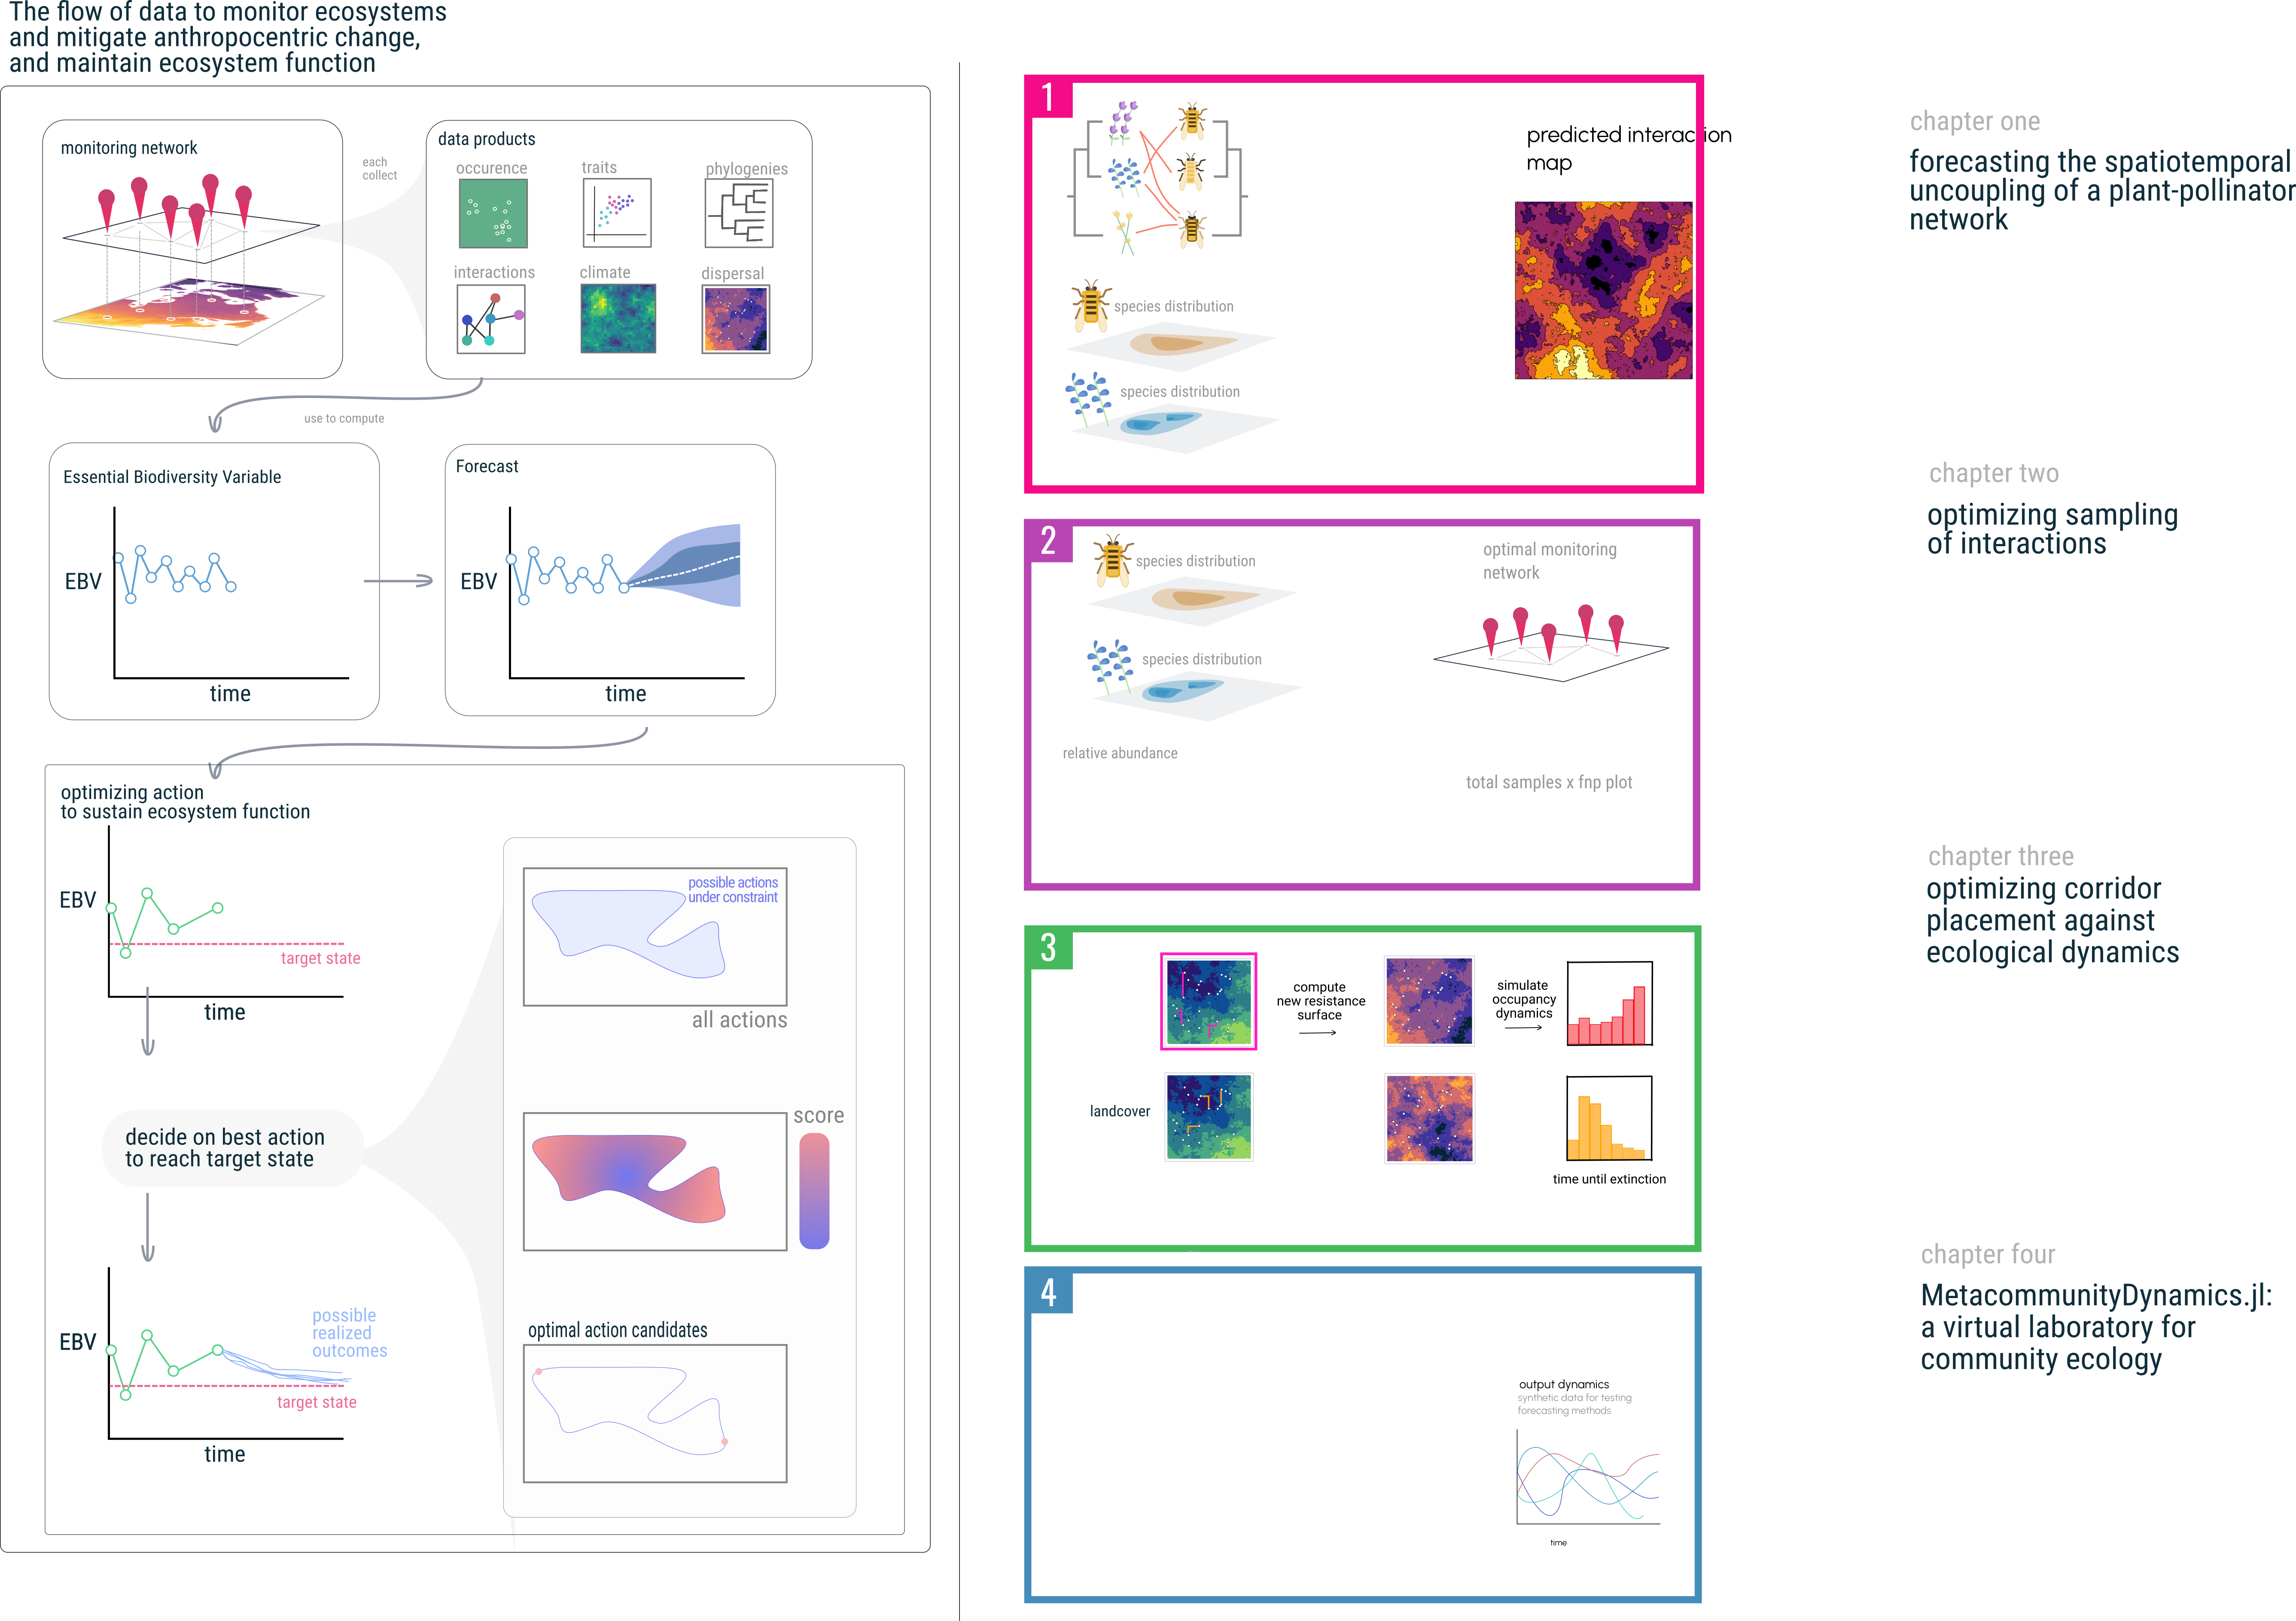
\includegraphics{./figures/thesisconcept.png}
\caption{thesis concept}\label{fig:thesis}
}
\end{figure}

\hypertarget{chapter-one-forecasting-the-spatial-uncoupling-of-a-plant-pollinator-network}{%
\section{Chapter One: Forecasting the spatial uncoupling of a
plant-pollinator
network}\label{chapter-one-forecasting-the-spatial-uncoupling-of-a-plant-pollinator-network}}

Interactions between plants and pollinators form networks of
interactions, which structure the ``architecture of biodiversity''
(\textbf{Jordano2007?}). The functioning and stability of ecosystems
emerge from these interactions, but antropogenic change threatens to
unravel and ``rewire'' these networks (\textbf{CaraDonna2017IntRew?}),
threating the persistence of these systems. Plant-pollinator networks
face two possible forms of rewiring in response to anthropogenic
environmental change: spatial and temporal. Spatially, range shifts
could cause interacting species to no longer overlap in space, and
shifts in phenology could cause interacting species to no longer overlap
in time.

This chapter uses several years of data on bumblebee-flower phenology
and interactions across several field sites, each consisting of several
plots across an elevational gradient, combined with spatial records of
species occurrence via GBIF to forecast this uncoupling. This addresses
the EBV to forecast of EBV element of the flow from data to mitigation
in fig.~\ref{fig:thesis} (left).

\begin{figure}
\centering
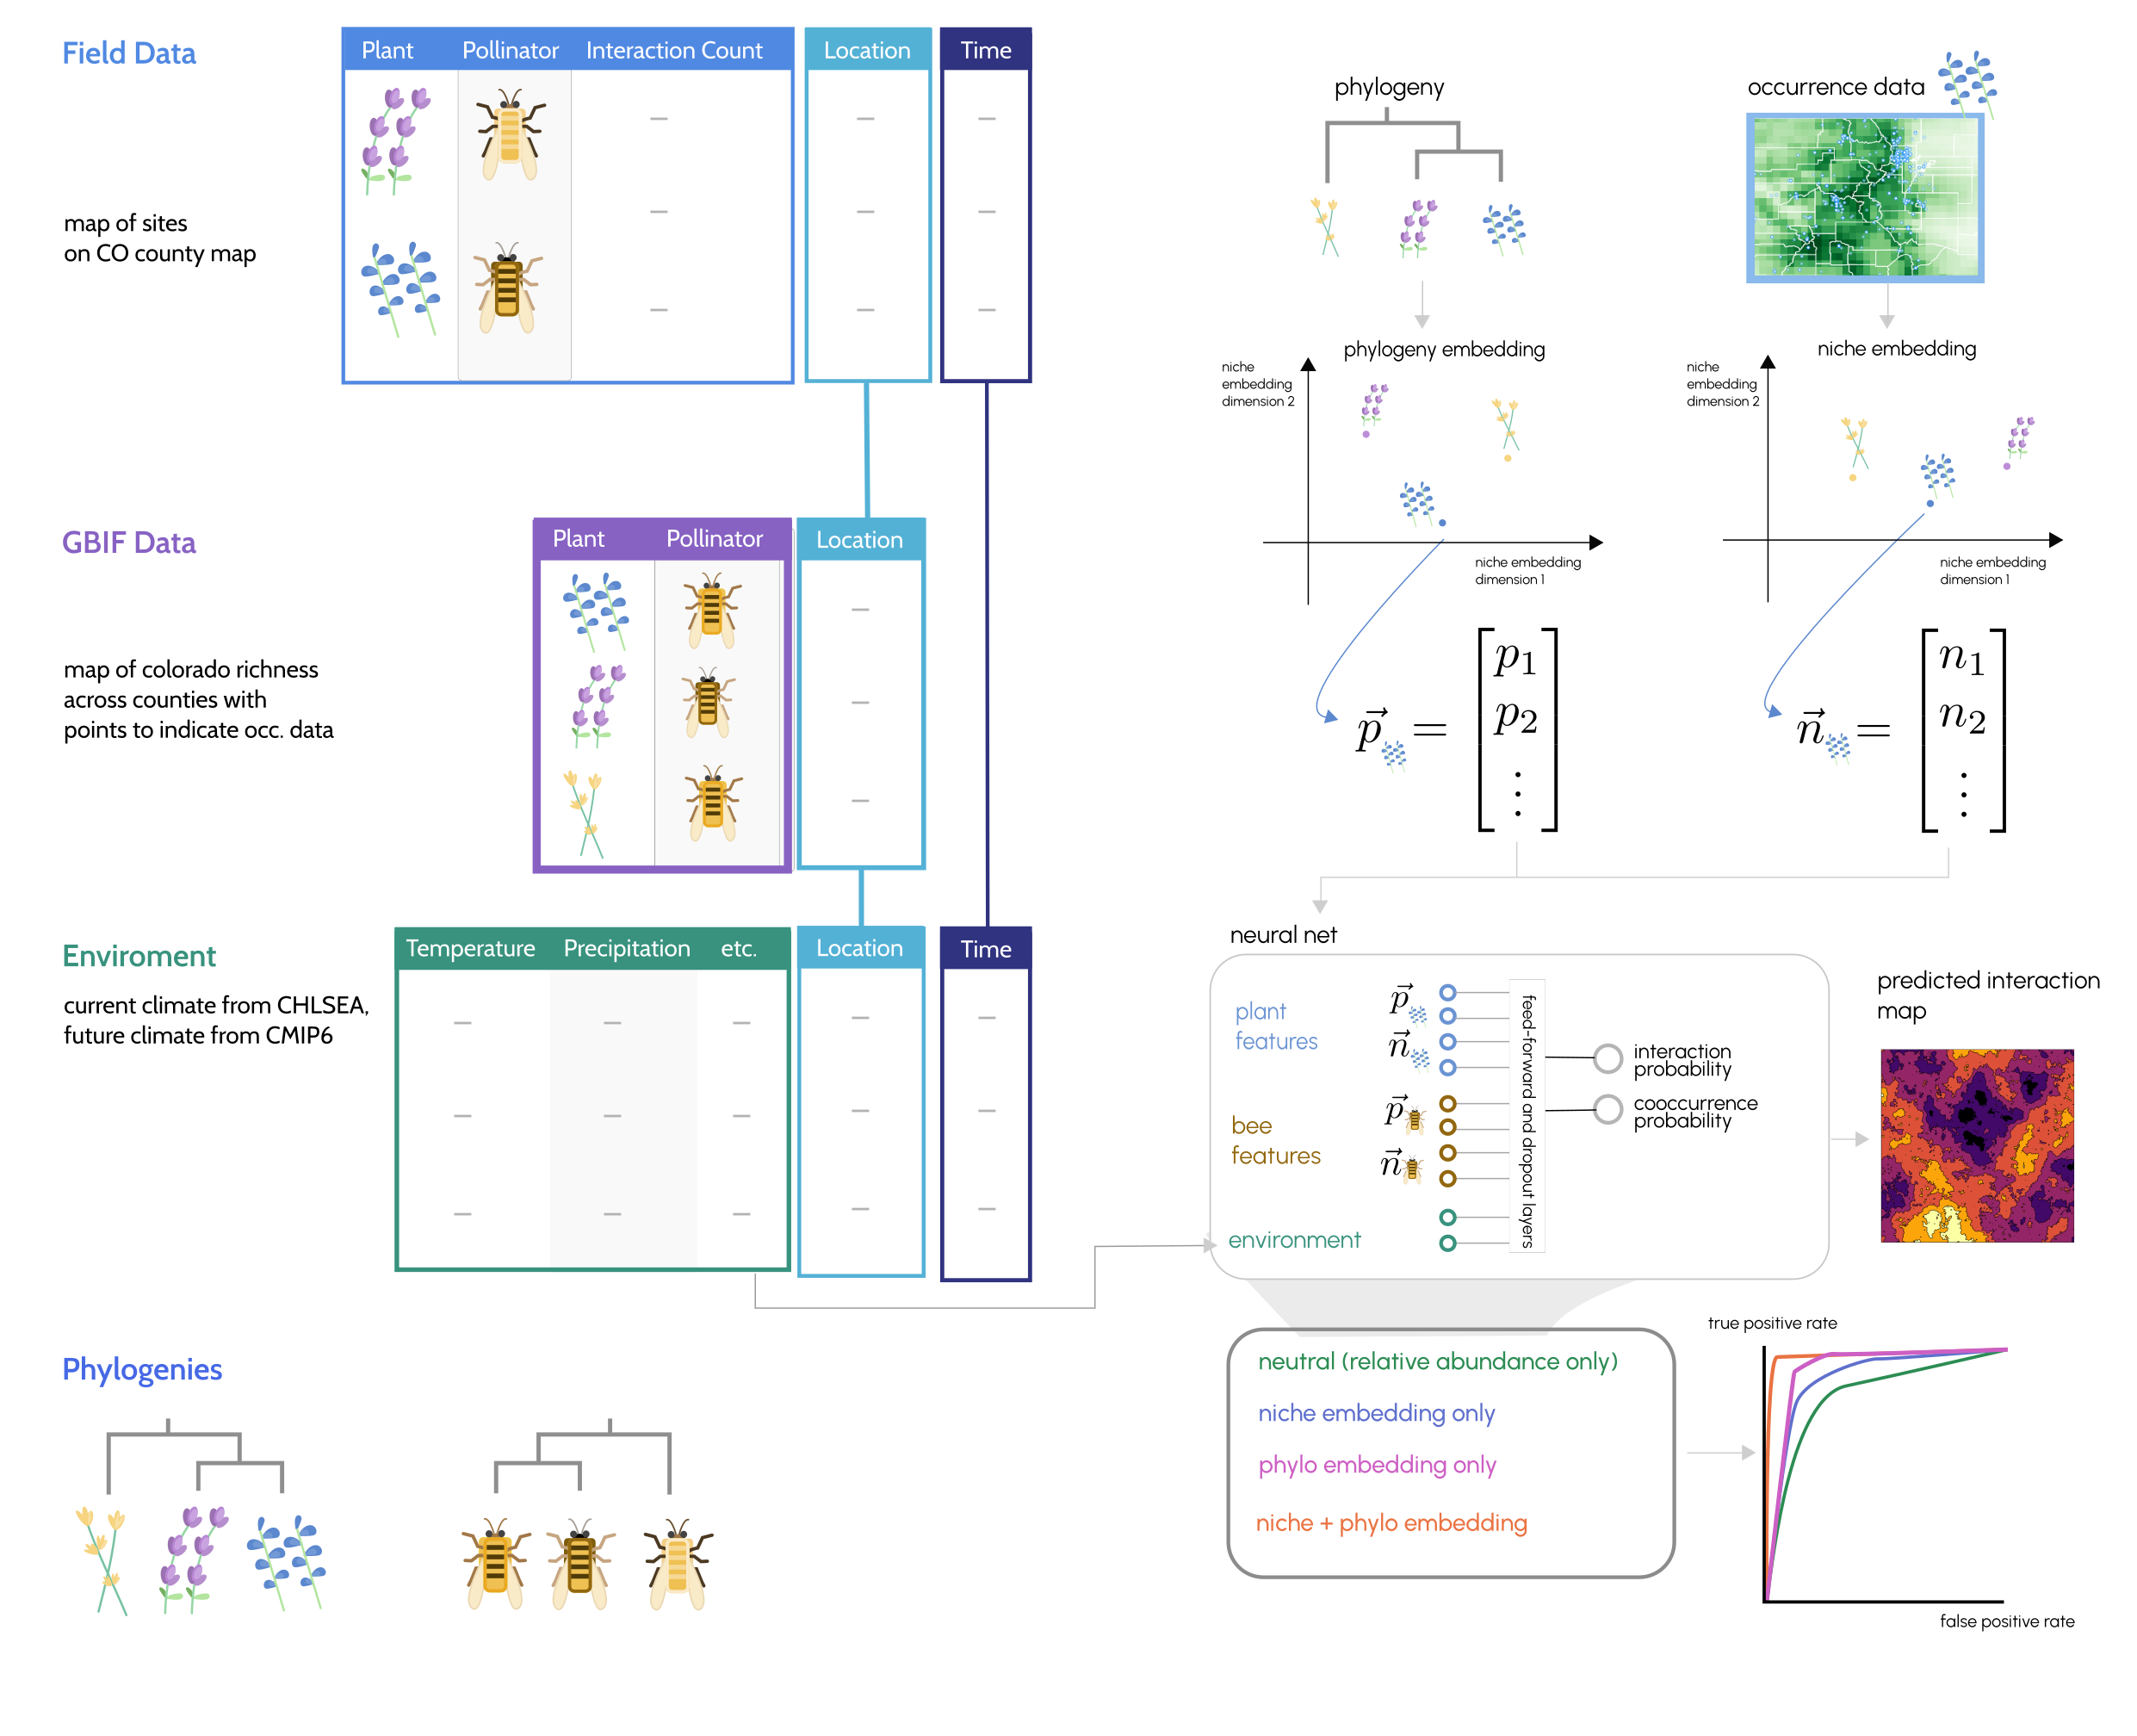
\includegraphics{./figures/ch1.png}
\caption{chapter one concept fig}
\end{figure}

\hypertarget{data}{%
\subsection{Data}\label{data}}

The data for this chapter is derived from multiple souces and can be
split into four categories. (1) Field data from three different field
sites across Colorado, each with multiple plots across an elevational
gradient, for seven, seven, and three years resptively. This data was
collected by Paul CaraDonna and Jane Oglevie (from the Rocky Mountain
Biological Laboratory) and Julian Resasco (CU Boulder). (2) GBIF spatial
occurrence records of each of these species across Colorado, including a
metaweb of interactions across all of Colroado taken from GBIF. (3)
Remotely sensed data consisting of current and forecasting bioclimatic
variables from CHELSA. (4) Phylogeny derived from NCBI GenBank barcodes
for mitochondrial COI (bumblebees) and chloroplast rbcL (flowers).

\hypertarget{methods}{%
\subsection{Methods}\label{methods}}

As the data we have is spatially sparse and likely to contain many
interaction ``false-negatives'' (Strydom \emph{et al.} 2021), we beign
by predicting a metaweb of interactions as they exist \emph{in the
present}.

In stages, (1) take data from multiple sites to predict a spatial
metaweb of \emph{Bombus}-flower interactions across Colorado. (2)
Predict how these spatial distributions will change under CMIP6. and (3)
quantify the lack of overlap between species for which there is a
predicted

The process of going from data to forecast can be split into the
following parts

\begin{enumerate}
\def\labelenumi{\arabic{enumi})}
\tightlist
\item
  Building an interaction prediction model (or rather a set of candidate
  models, relative abundance, phylo embedding relative abundance + phylo
  embedding) a la Strydom \emph{et al.} (2021)
\end{enumerate}

Reconstructing latent features for each species based on simulating
trait evolution on a phylogeny (\textbf{Strydom2021FooWeb?}).

\begin{enumerate}
\def\labelenumi{\arabic{enumi})}
\setcounter{enumi}{1}
\item
  Make it spatial based on distributions.
\item
  Forecast distributions based on CMIP6
\end{enumerate}

\hypertarget{preliminary-results}{%
\subsection{Preliminary Results}\label{preliminary-results}}

\begin{enumerate}
\def\labelenumi{\arabic{enumi})}
\tightlist
\item
  we got a tree and SDMs
\end{enumerate}

Transition to next chapter by discussing uncertainty in interaction
prediction across space.

\hypertarget{chapter-two-optimizing-spatial-sampling-of-species-interactions}{%
\section{Chapter Two: Optimizing spatial sampling of species
interactions}\label{chapter-two-optimizing-spatial-sampling-of-species-interactions}}

This chapter uses simulation models to investigate the relationship
between species relative abundance, sampling effort, and probability of
accurately detecting an interaction between species, and further
proposes a method for optimizing the spatial sampling locations to
maximize the probability of detecting an interaction between two species
given their distributions. This addresses the optimization of monitoring
network part of the flow from data to mitigation in
fig.~\ref{fig:thesis}.

As explored in the previous chapter, there are false-negatives in
interation data. There is more than one way to observe a false-negative
when sampling interactions: (fig.~\ref{fig:fnrtaxonomy}). It begins with
a conceptual framework for understanding the difference in
false-negatives in occurrence, co-occurrence, and interactions.
Co-occurrence is not the same thing as interaction (Blanchet \emph{et
al.} 2020), but often is used as a proxy.

\begin{figure}
\hypertarget{fig:fnrtaxonomy}{%
\centering
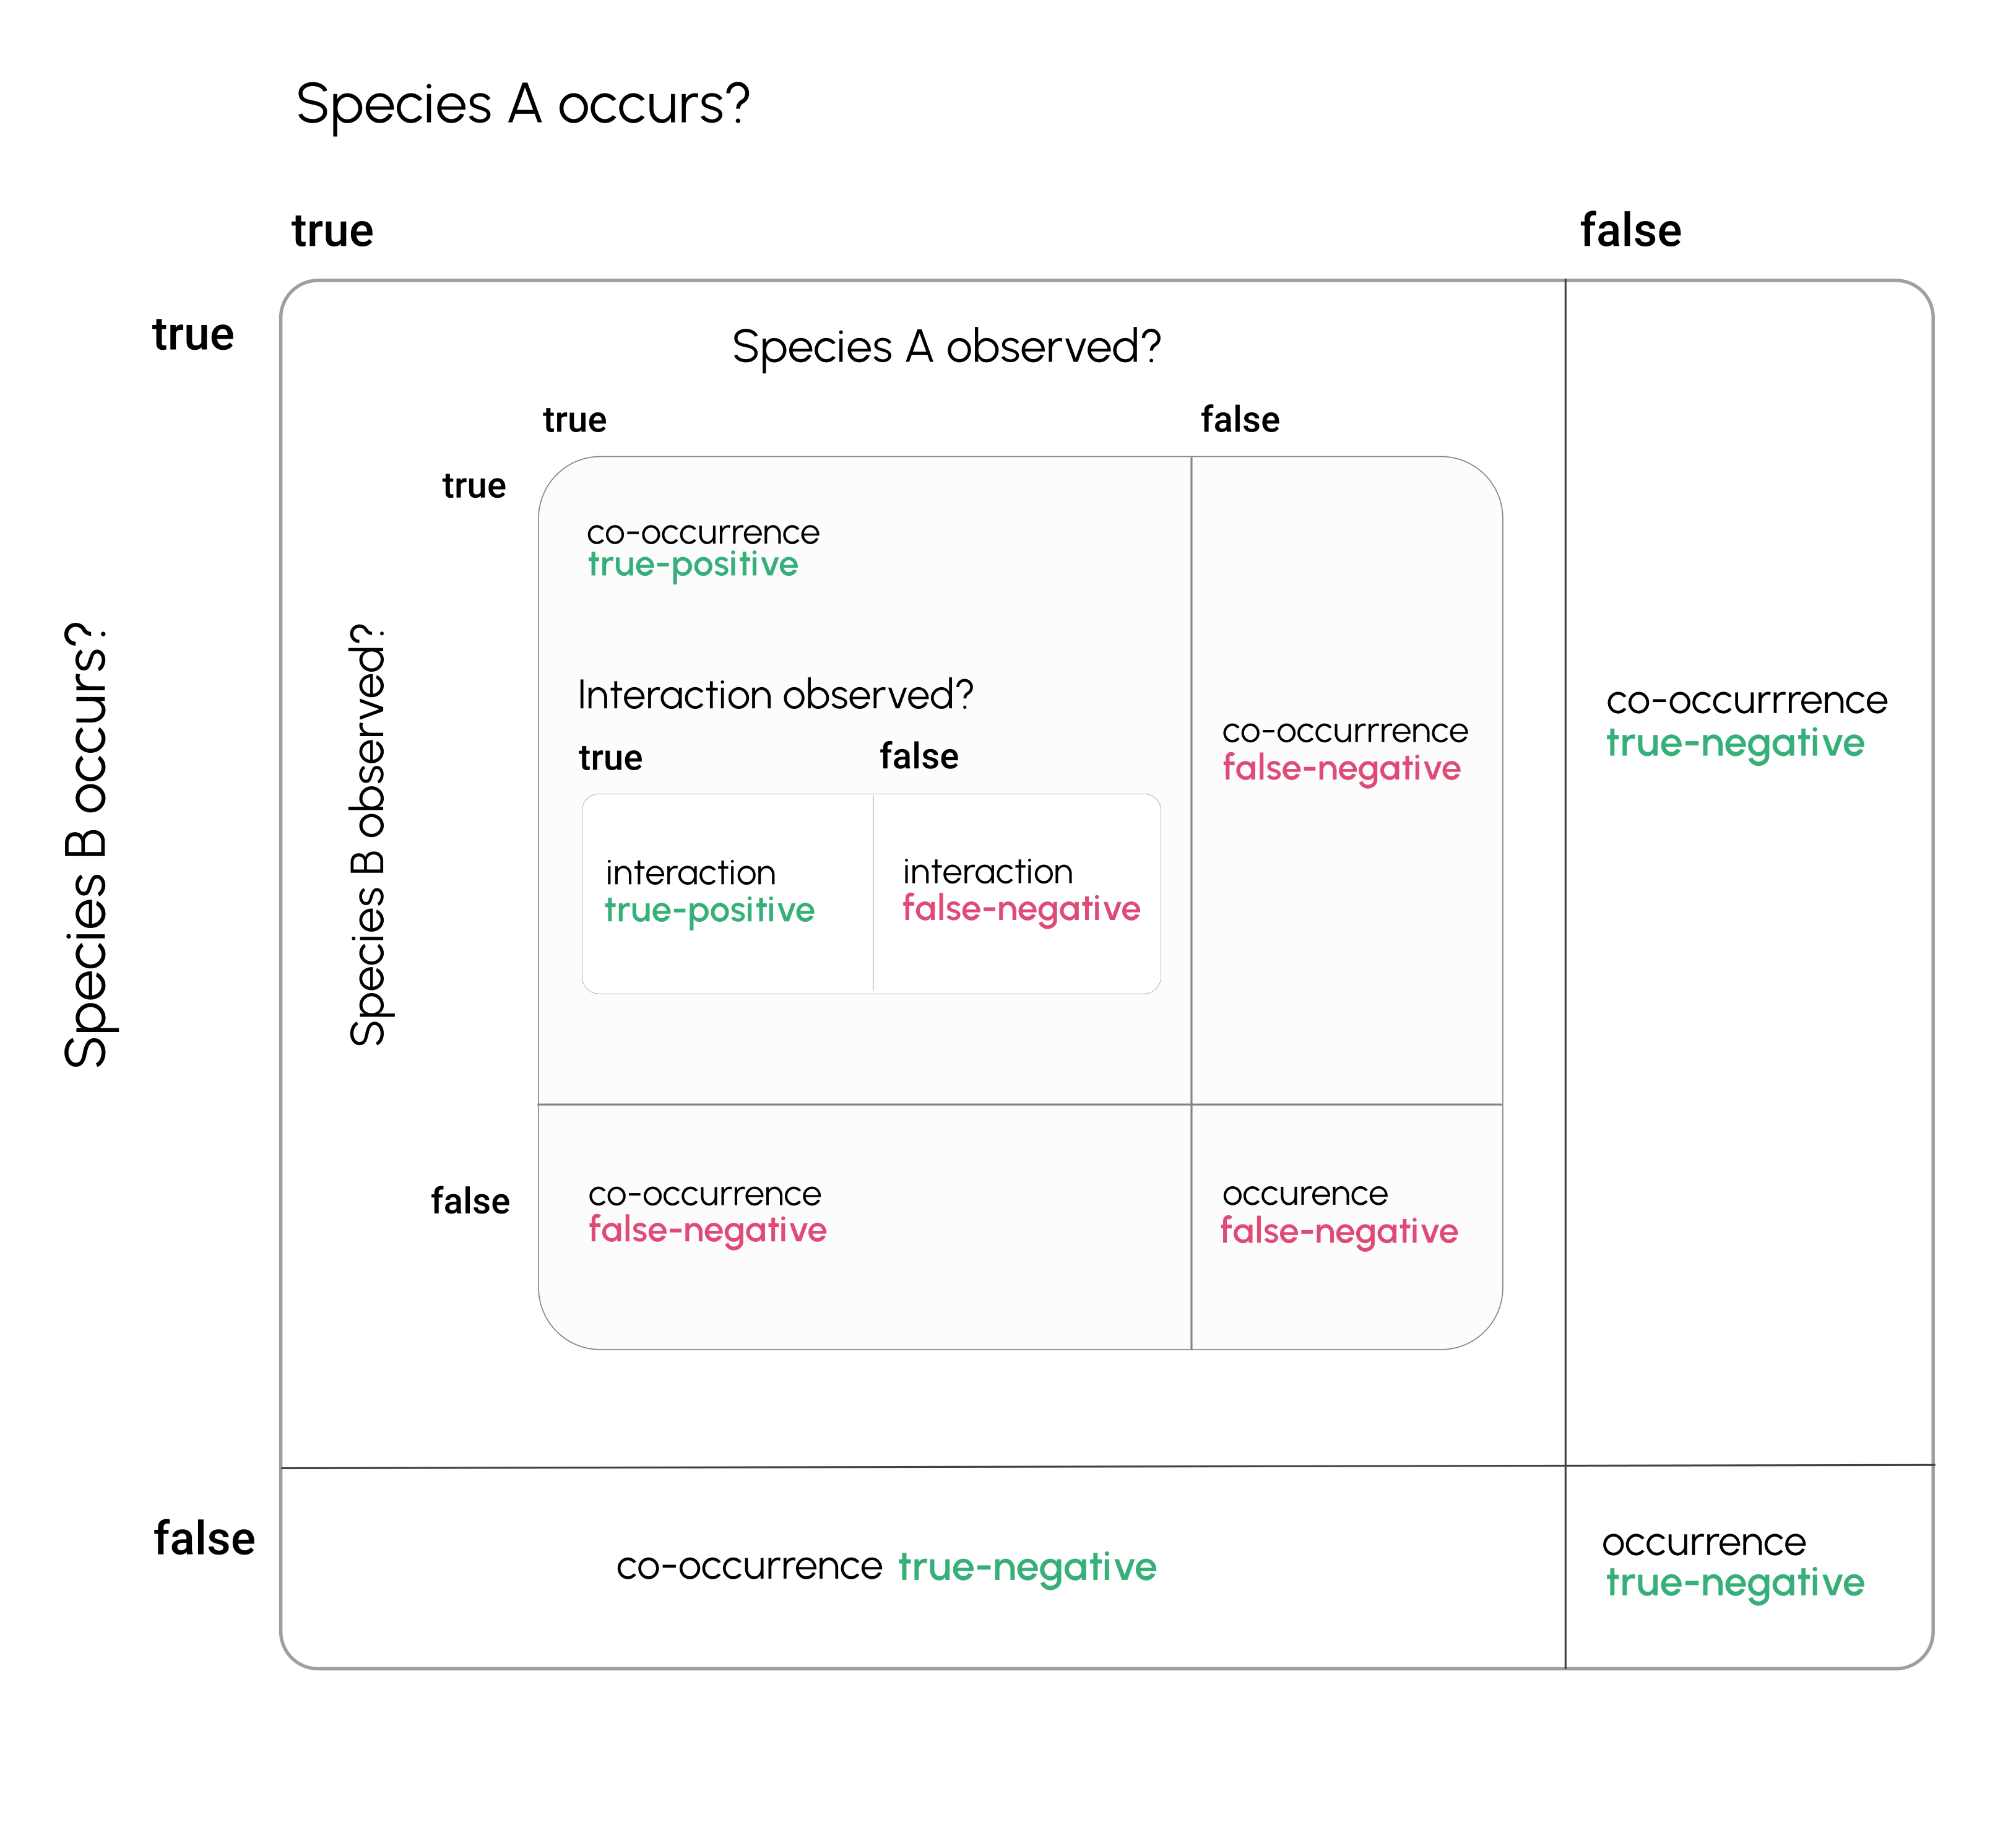
\includegraphics{./figures/ch2.png}
\caption{taxonomy of false negatives}\label{fig:fnrtaxonomy}
}
\end{figure}

We use a log-normal distribution as a null model of the
relative-abundance distribution (Hubbell 2001) to simulate realized
false-negative rate as a function of varying sampling effort.

This also goes on to includes testing some assumptions of the model with
empirical data fig.~\ref{fig:posassoc}, which we analytically show that
our neutral model, if anything, underestimates the probability of
false-negatives due to positive correlations in co-occurrence in two
sets of spatially replicated samples of interaction networks (Thompson
\& Townsend 2000; Hadfield \emph{et al.} 2014)---further I'm planning to
add the field data from the previous chapter into this anlysis once
available.

\begin{figure}
\hypertarget{fig:posassoc}{%
\centering
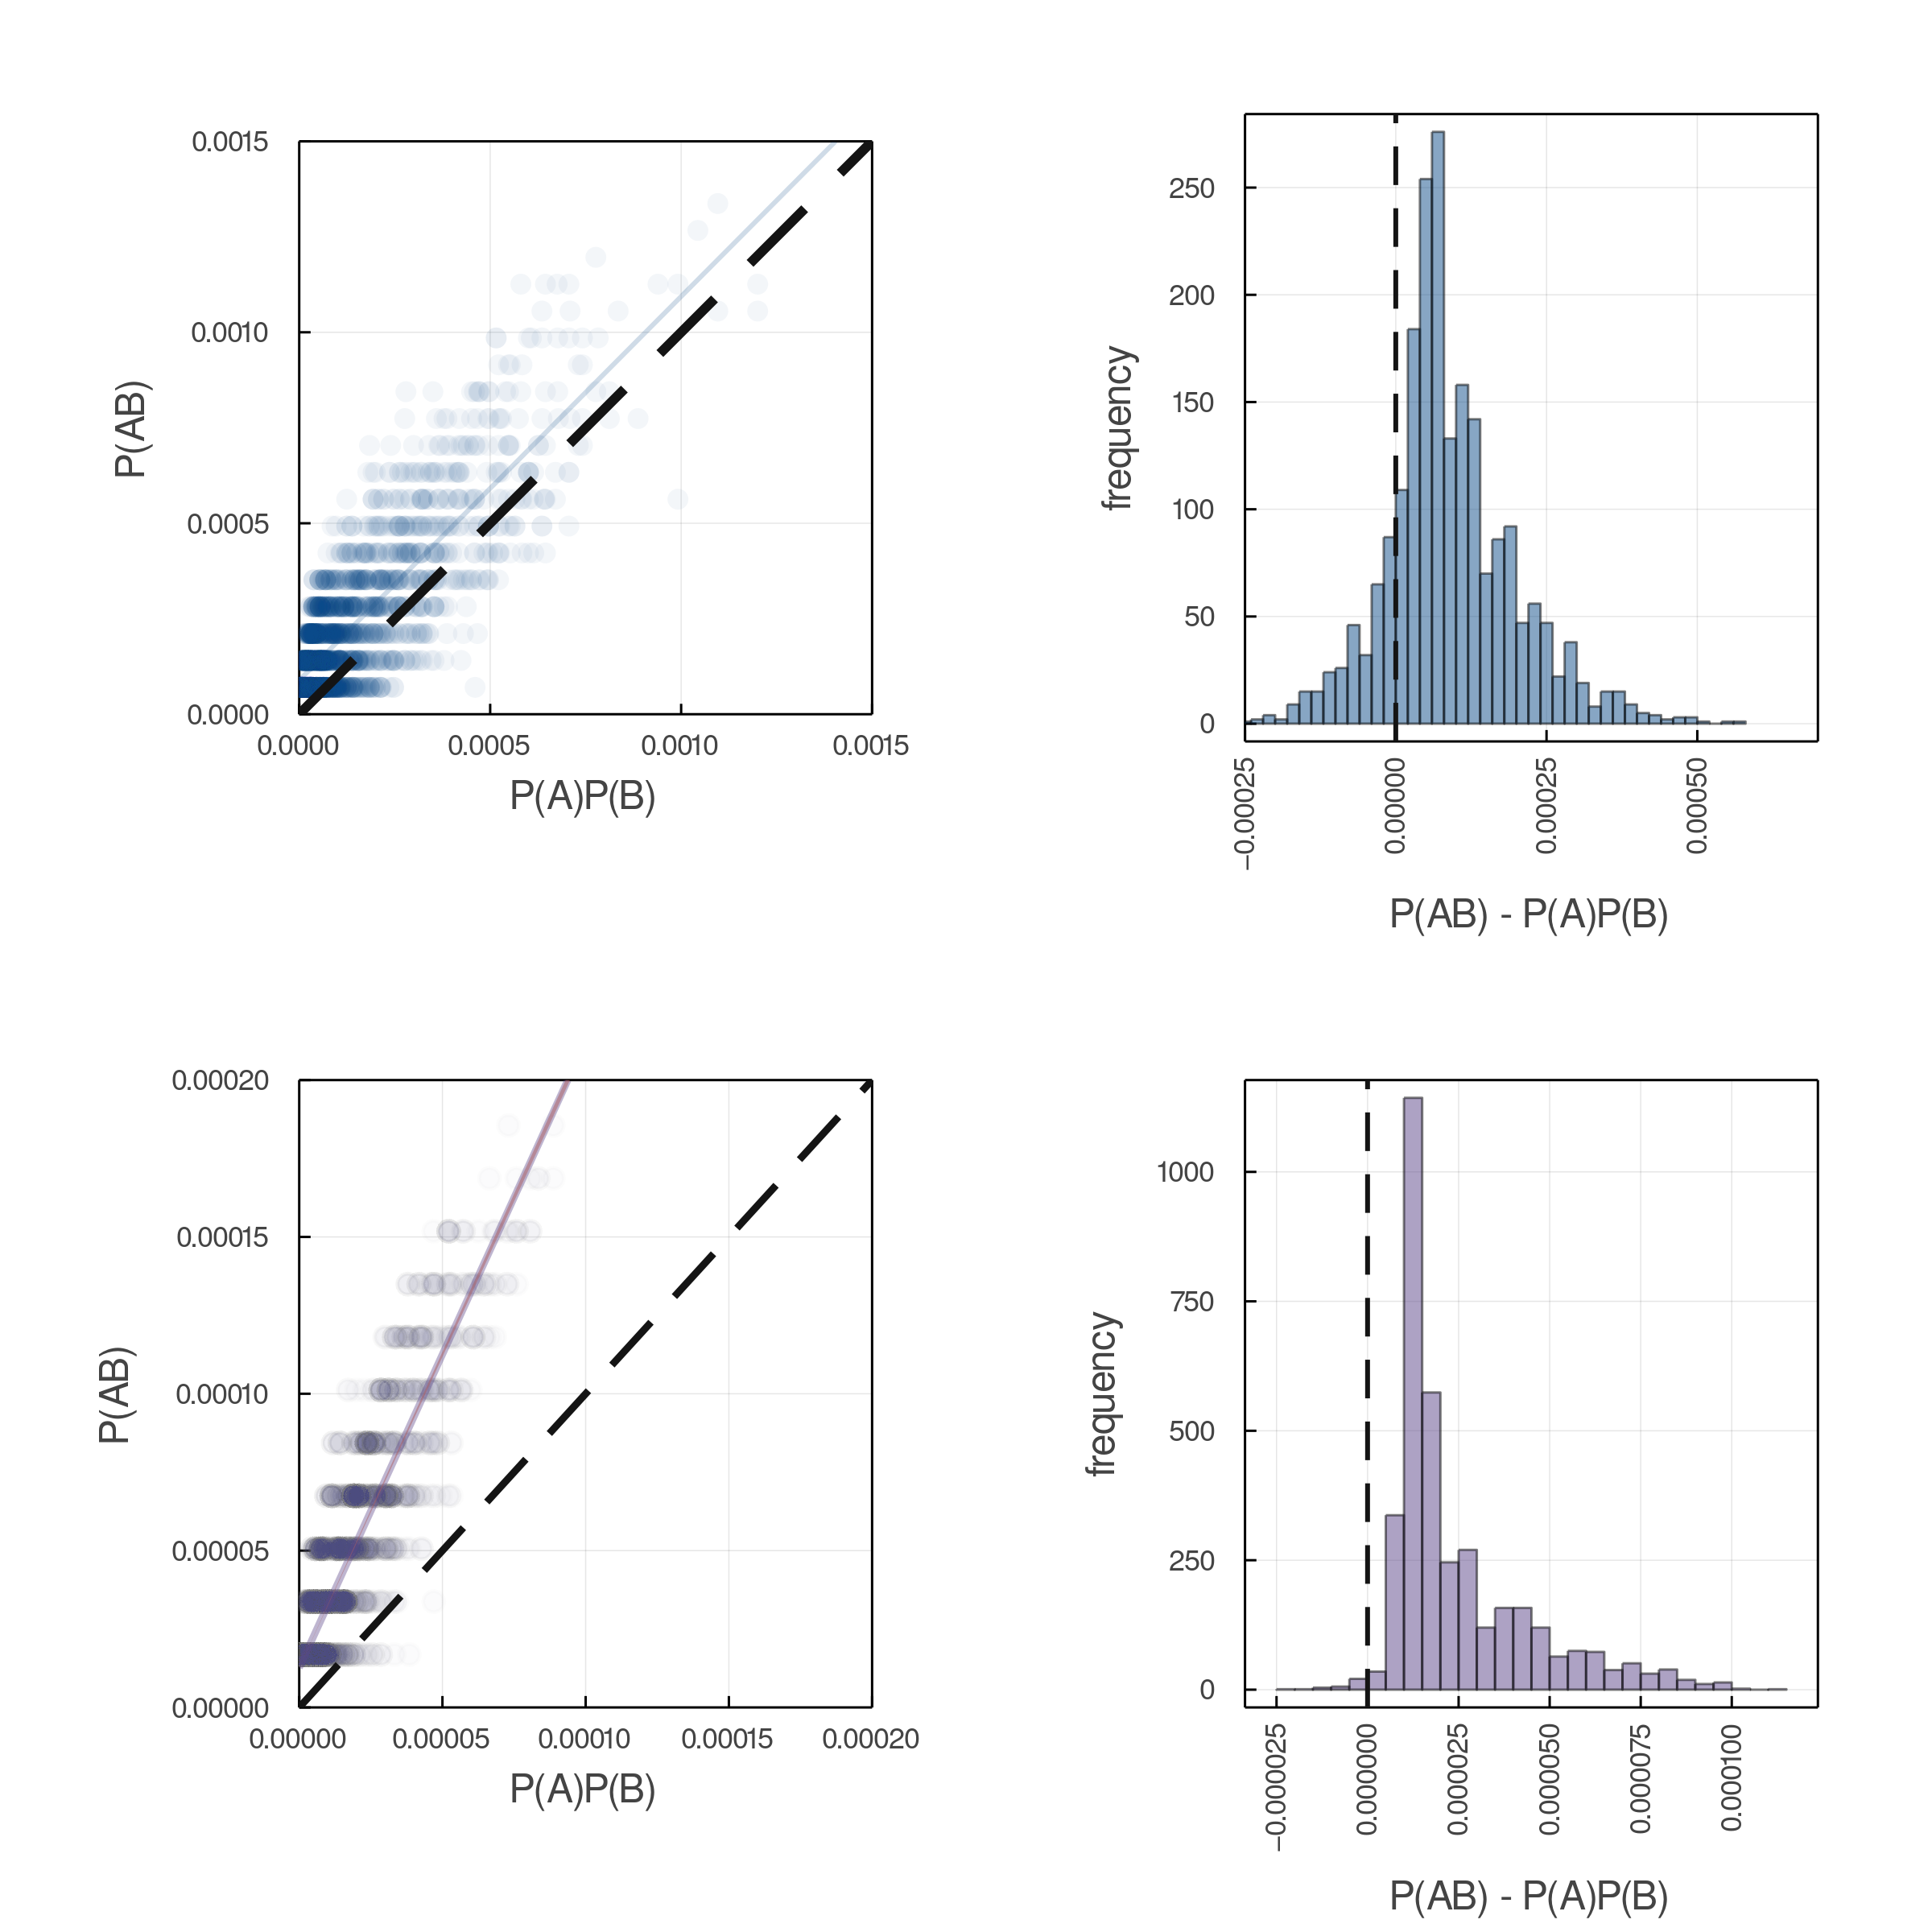
\includegraphics{./figures/positiveassociations.png}
\caption{f}\label{fig:posassoc}
}
\end{figure}

Finally this chapter proposes a simulated annealing method to optimize
the efficacy of interactoin detection given a set of observation points
where the dist from observation site decays. optimize set of repeated
sampling locations L for a pair of species \emph{known} distributions
\(D_a, D_b\).

\hypertarget{chapter-three-optimizing-corridor-placement-against-ecological-dynamics}{%
\section{Chapter Three: Optimizing corridor placement against ecological
dynamics}\label{chapter-three-optimizing-corridor-placement-against-ecological-dynamics}}

Promoting landscape connectivity is important to mitigate the effects of
land-use change on Earth's biodiversity. However, the practical
realities of conservation mean that there is a limitation on how much we
can modify landscapes in order to do this. So what is the best place to
put a corridor given a constraint on how much surface-area you can
change in a landscape? This is the question this chapter seeks to
answer. Models for proposing corridor locations have been developed, but
are limited in that are not developed around promoting some element of
ecosystem function, but instead by trying to find the path of least
resistance given a resistance surface (Peterman 2018).

This chapter proposes a general algorithm for choosing corridor
placement to optimize a measurement of ecosystem functioning derived
from simulations run on each proposed landscape modification.

\begin{figure}
\hypertarget{fig:ch3}{%
\centering
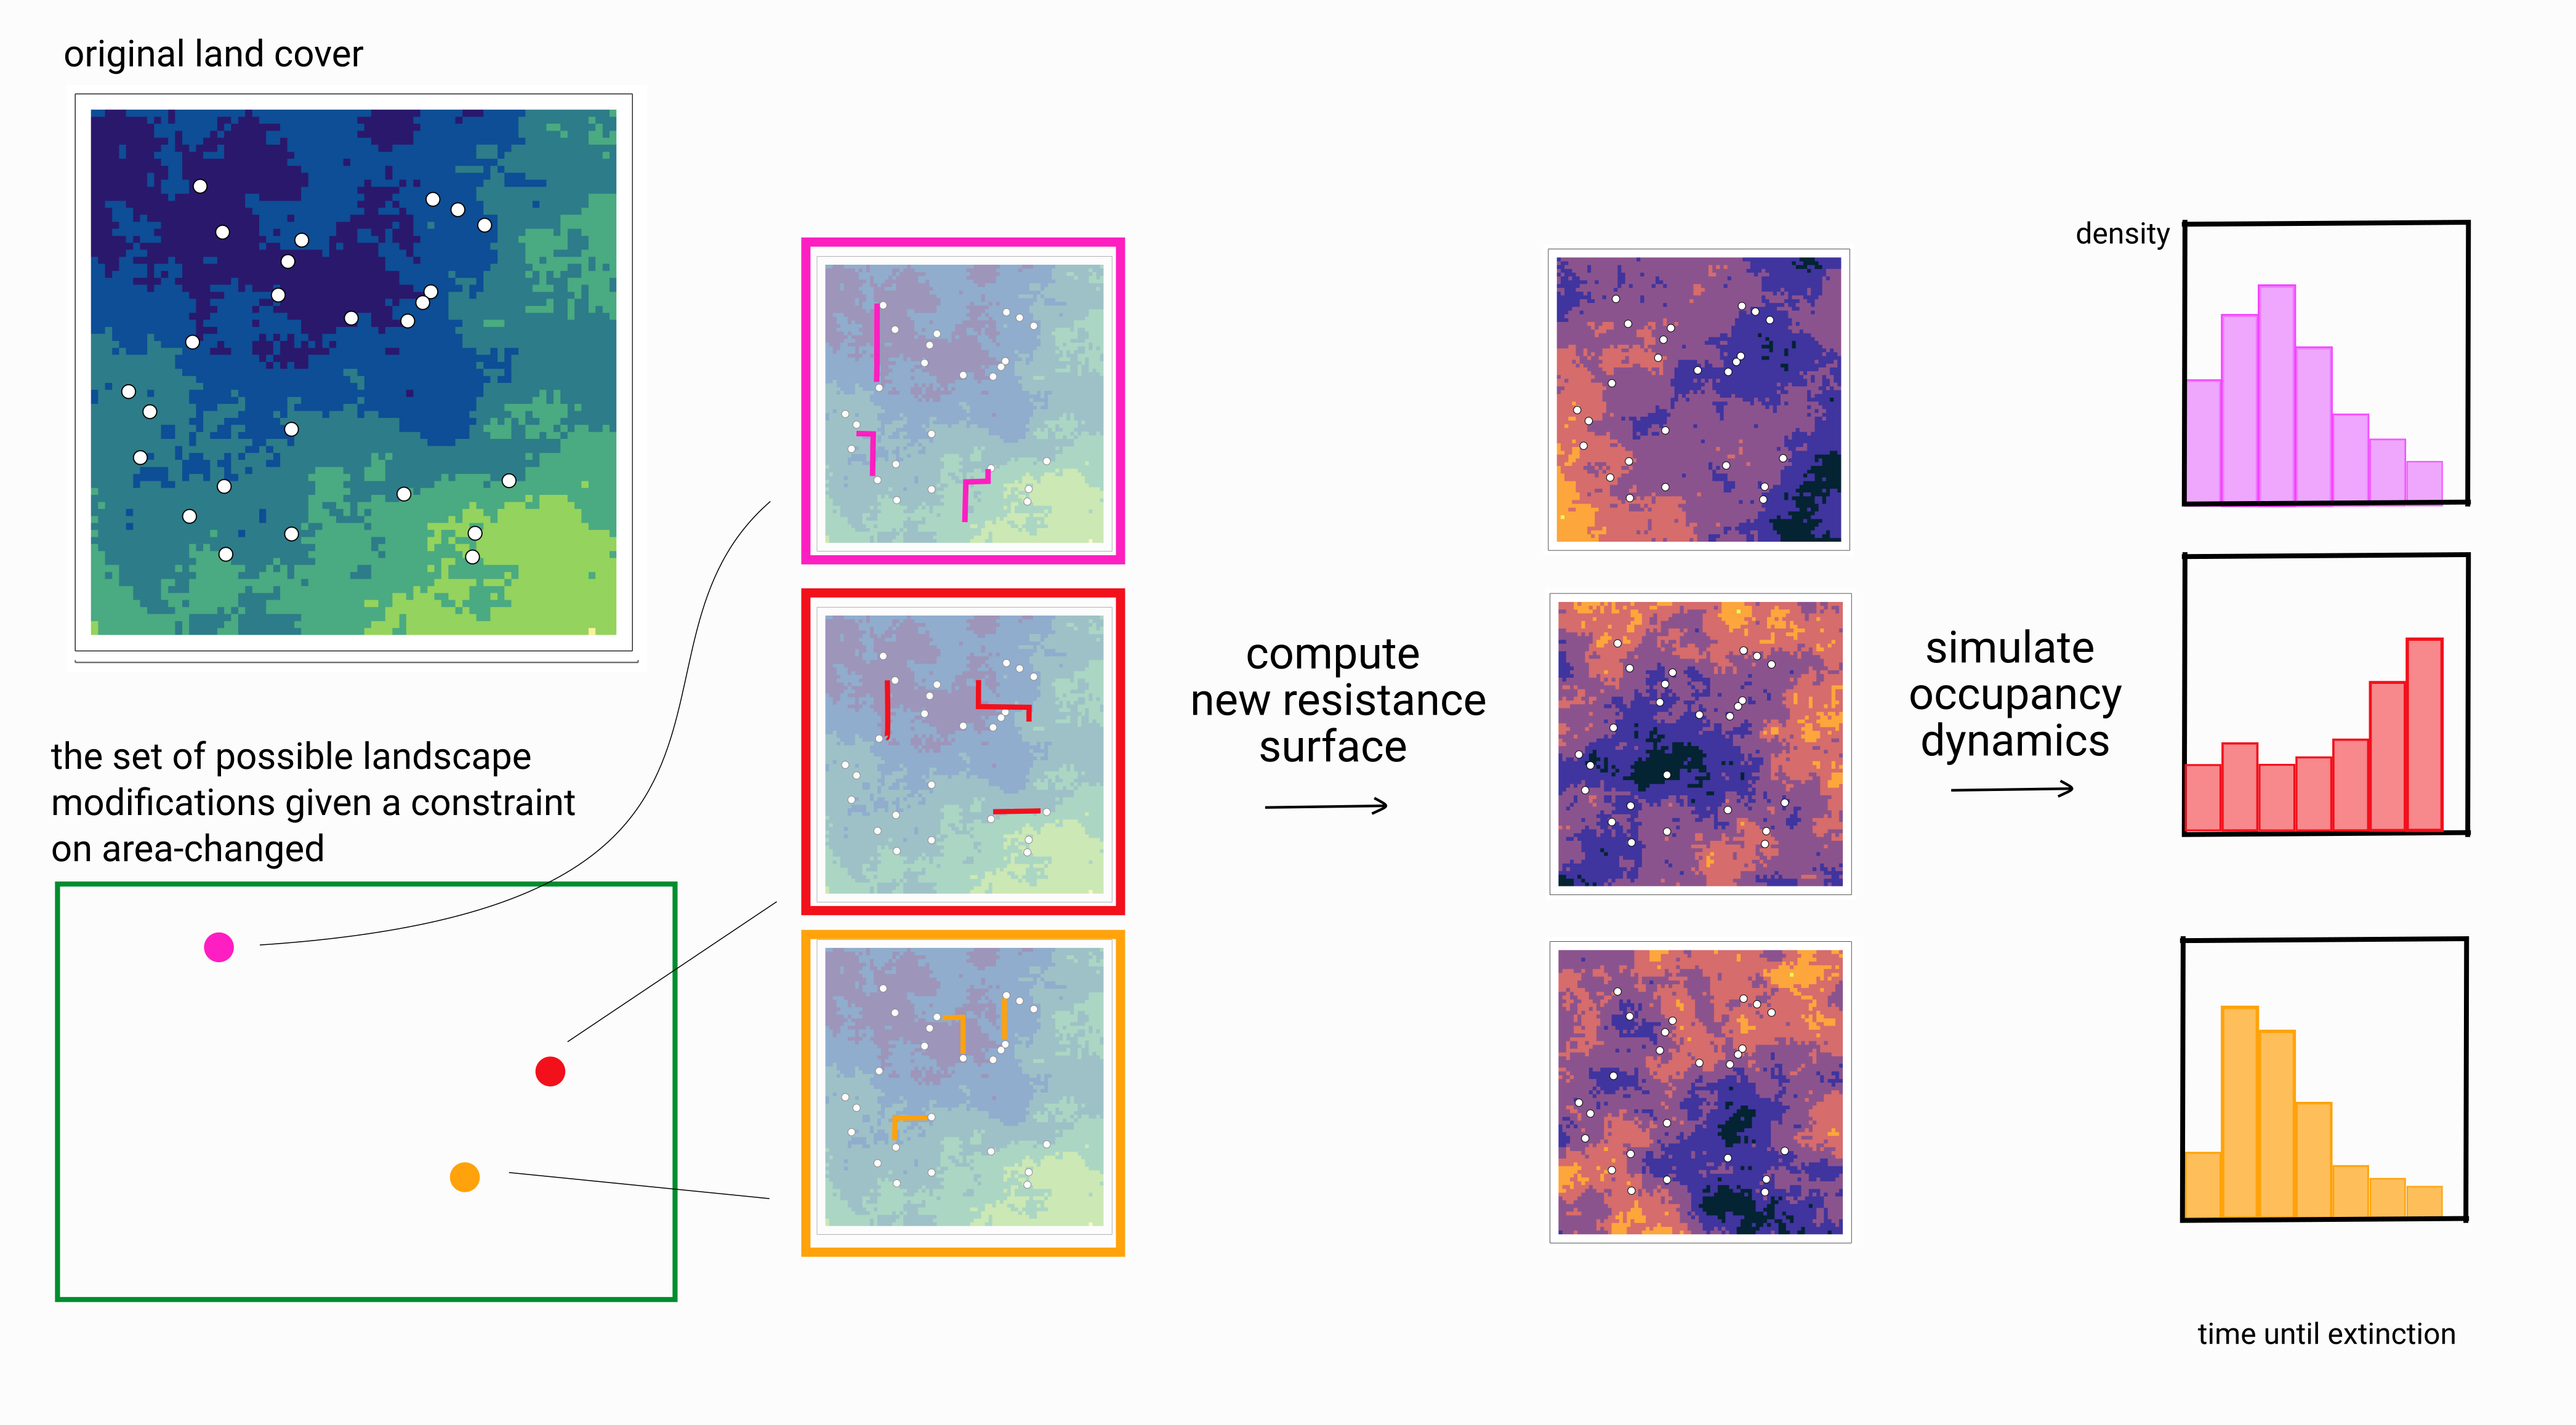
\includegraphics{./figures/ch3.png}
\caption{fig}\label{fig:ch3}
}
\end{figure}

\hypertarget{methods-1}{%
\subsection{Methods}\label{methods-1}}

We propose various landscape modifications which alter the cover of a
landscape, represented as a raster. We then compute a new resistance
surface based on the proposed landscape modification, and based on the
values of resistance to dispersal between each location we simulate
spatially-explicit metapopulation dynamics model (Hanski \& Ovaskainen
2000; Ovaskainen \emph{et al.} 2002) to estimate a distribution of time
until extinction for each landscape modification.

\begin{itemize}
\tightlist
\item
  brief overview of simulated annealing describe how you build the
\item
  proposal function optimize landscape optimization
\end{itemize}

\hypertarget{chapter-four-metacommunitydynamics.jl-a-virtual-laboratory-for-community-ecology}{%
\section{Chapter Four: MetacommunityDynamics.jl: a virtual laboratory
for community
ecology}\label{chapter-four-metacommunitydynamics.jl-a-virtual-laboratory-for-community-ecology}}

This chapter consists of a collection of modules in the Julia language
for different aspects of community ecology, including most of the code
used for the preceding chapters. Indeed
\texttt{MetacommunityDynamics.jl} (MCD.jl) is the epicenter of this set
of tools, but due to the nature of the Julia language, MCD.jl is
interoperable with serveral existing packages within the
\texttt{EcoJulia} organization, including several to which I have
contributed. A diagram showing the relation between these packages is
shown in fig.~\ref{fig:software}.

\begin{figure}
\hypertarget{fig:software}{%
\centering
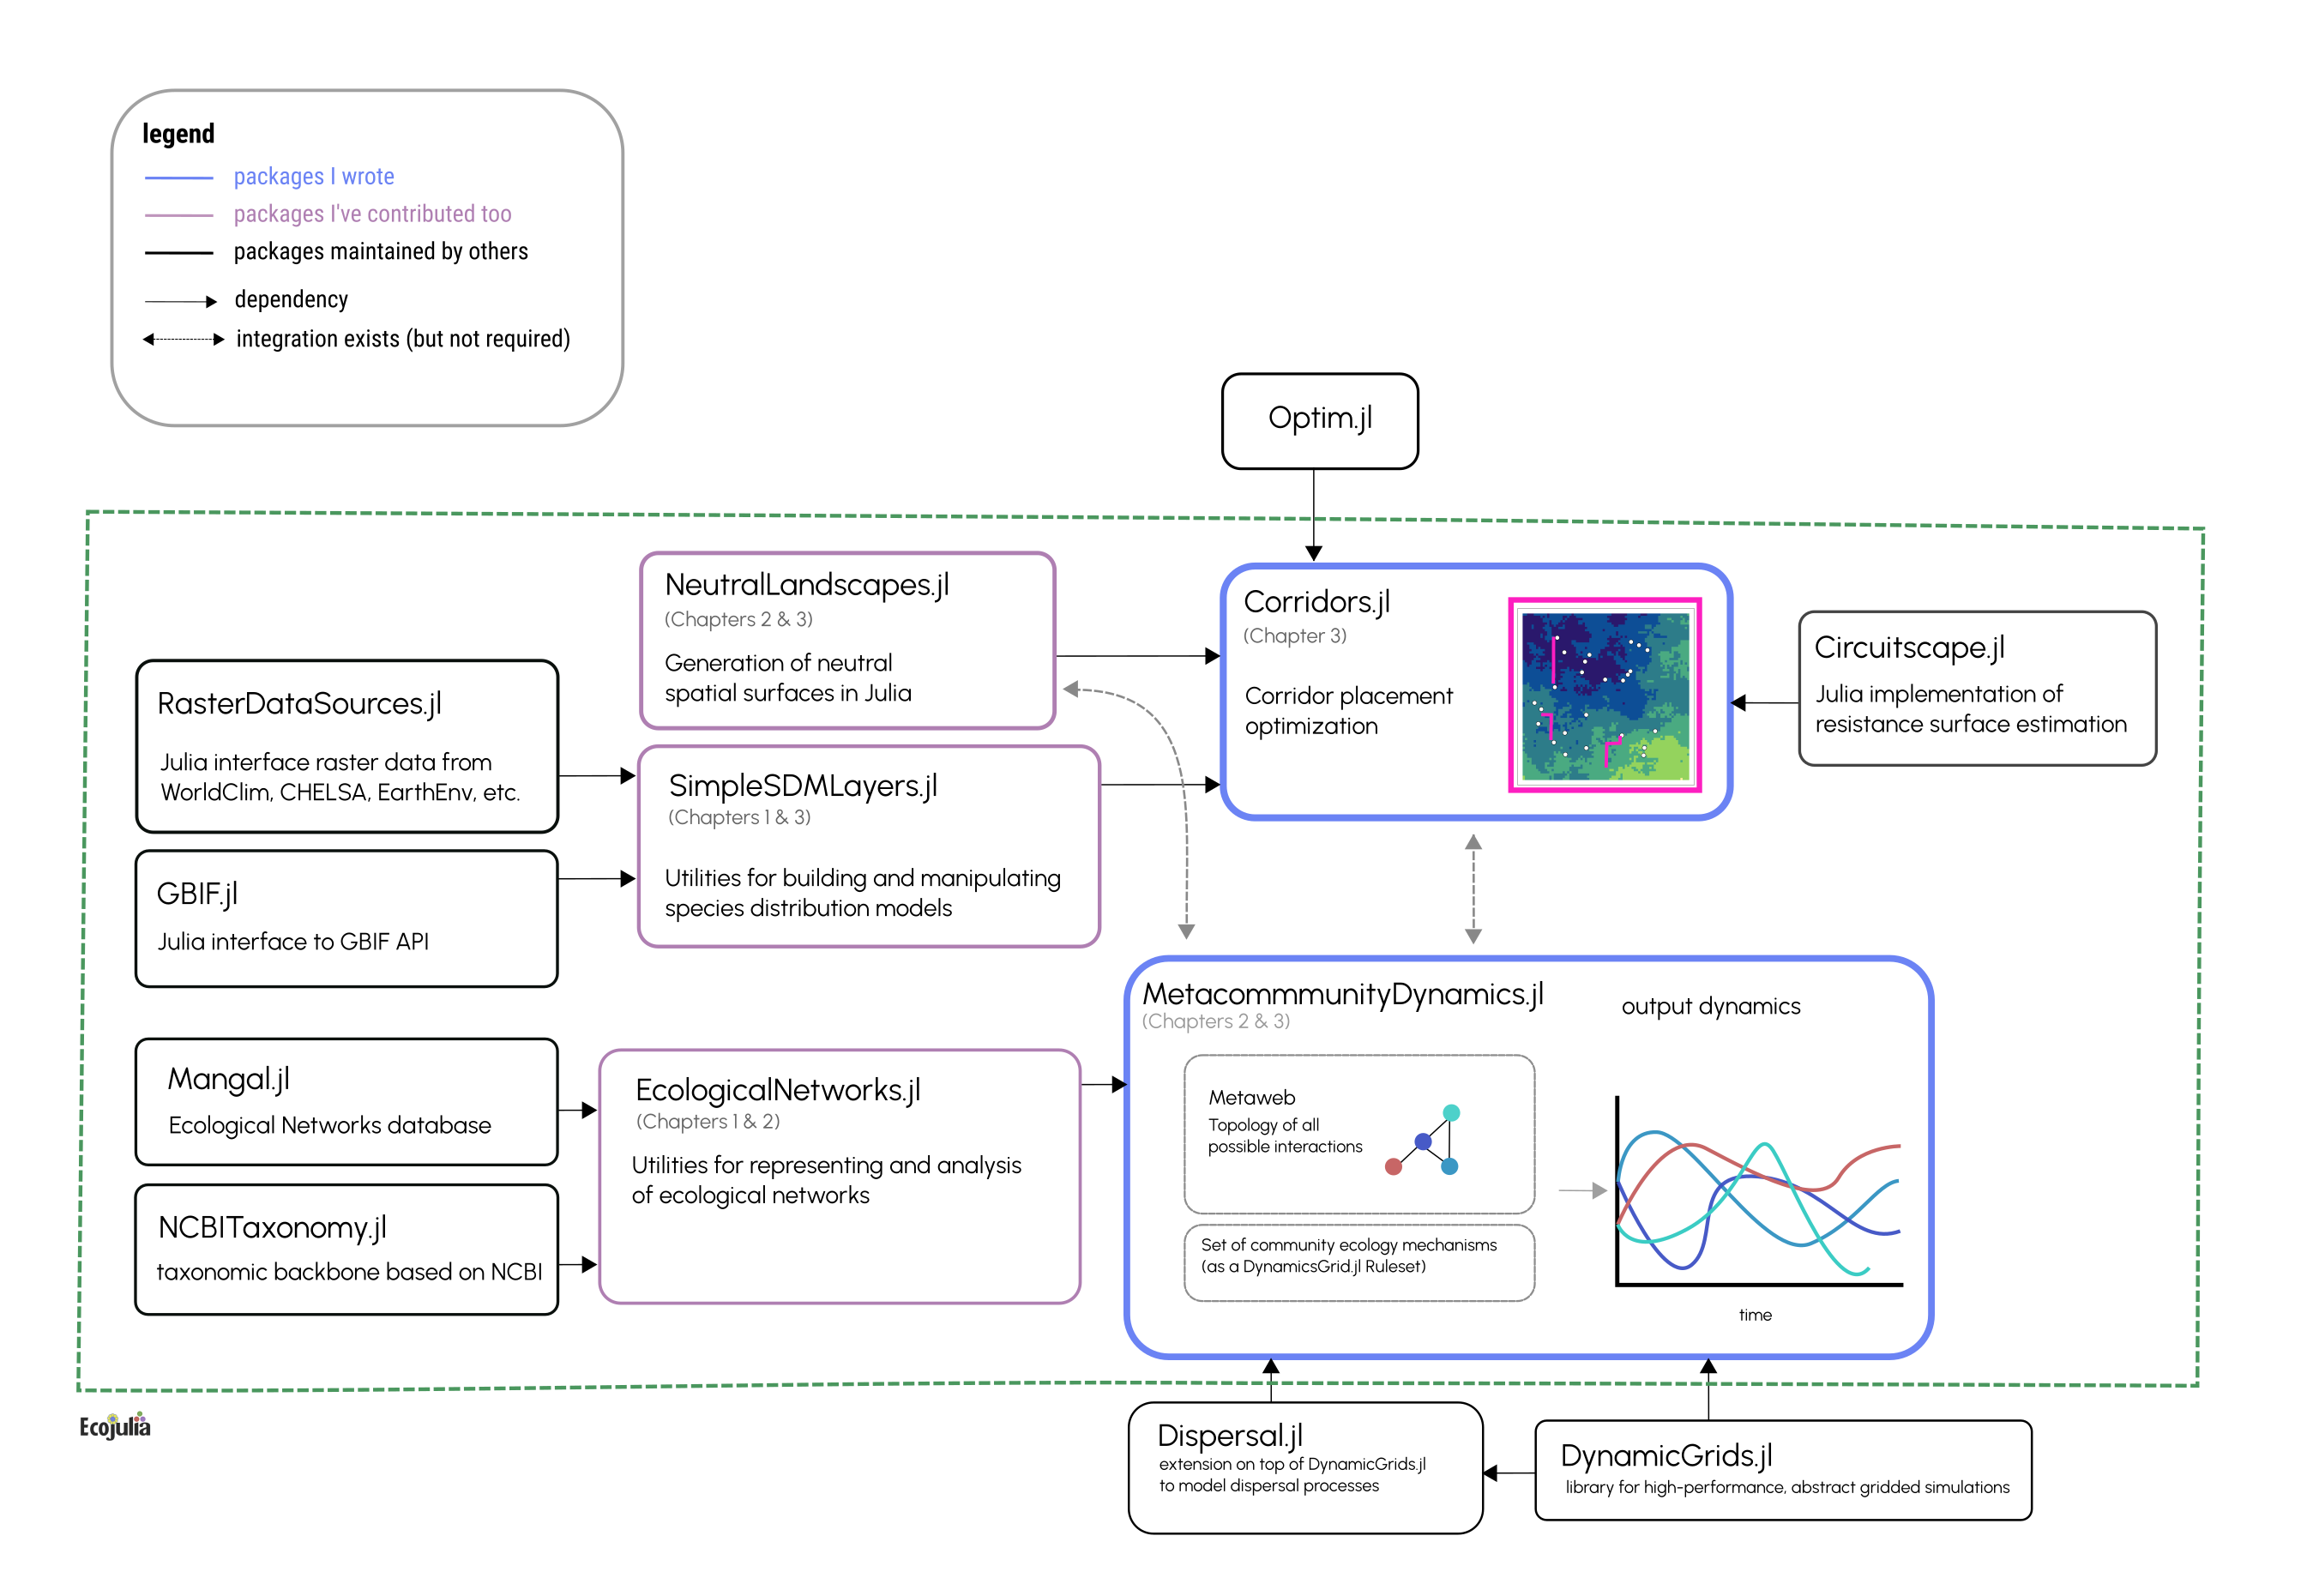
\includegraphics{./figures/ch4.png}
\caption{The structure of the software libraries used as part of
MCD.jl}\label{fig:software}
}
\end{figure}

\hypertarget{conclusion}{%
\section{Conclusion}\label{conclusion}}

\hypertarget{appendix}{%
\section{Appendix}\label{appendix}}

\begin{figure}
\centering
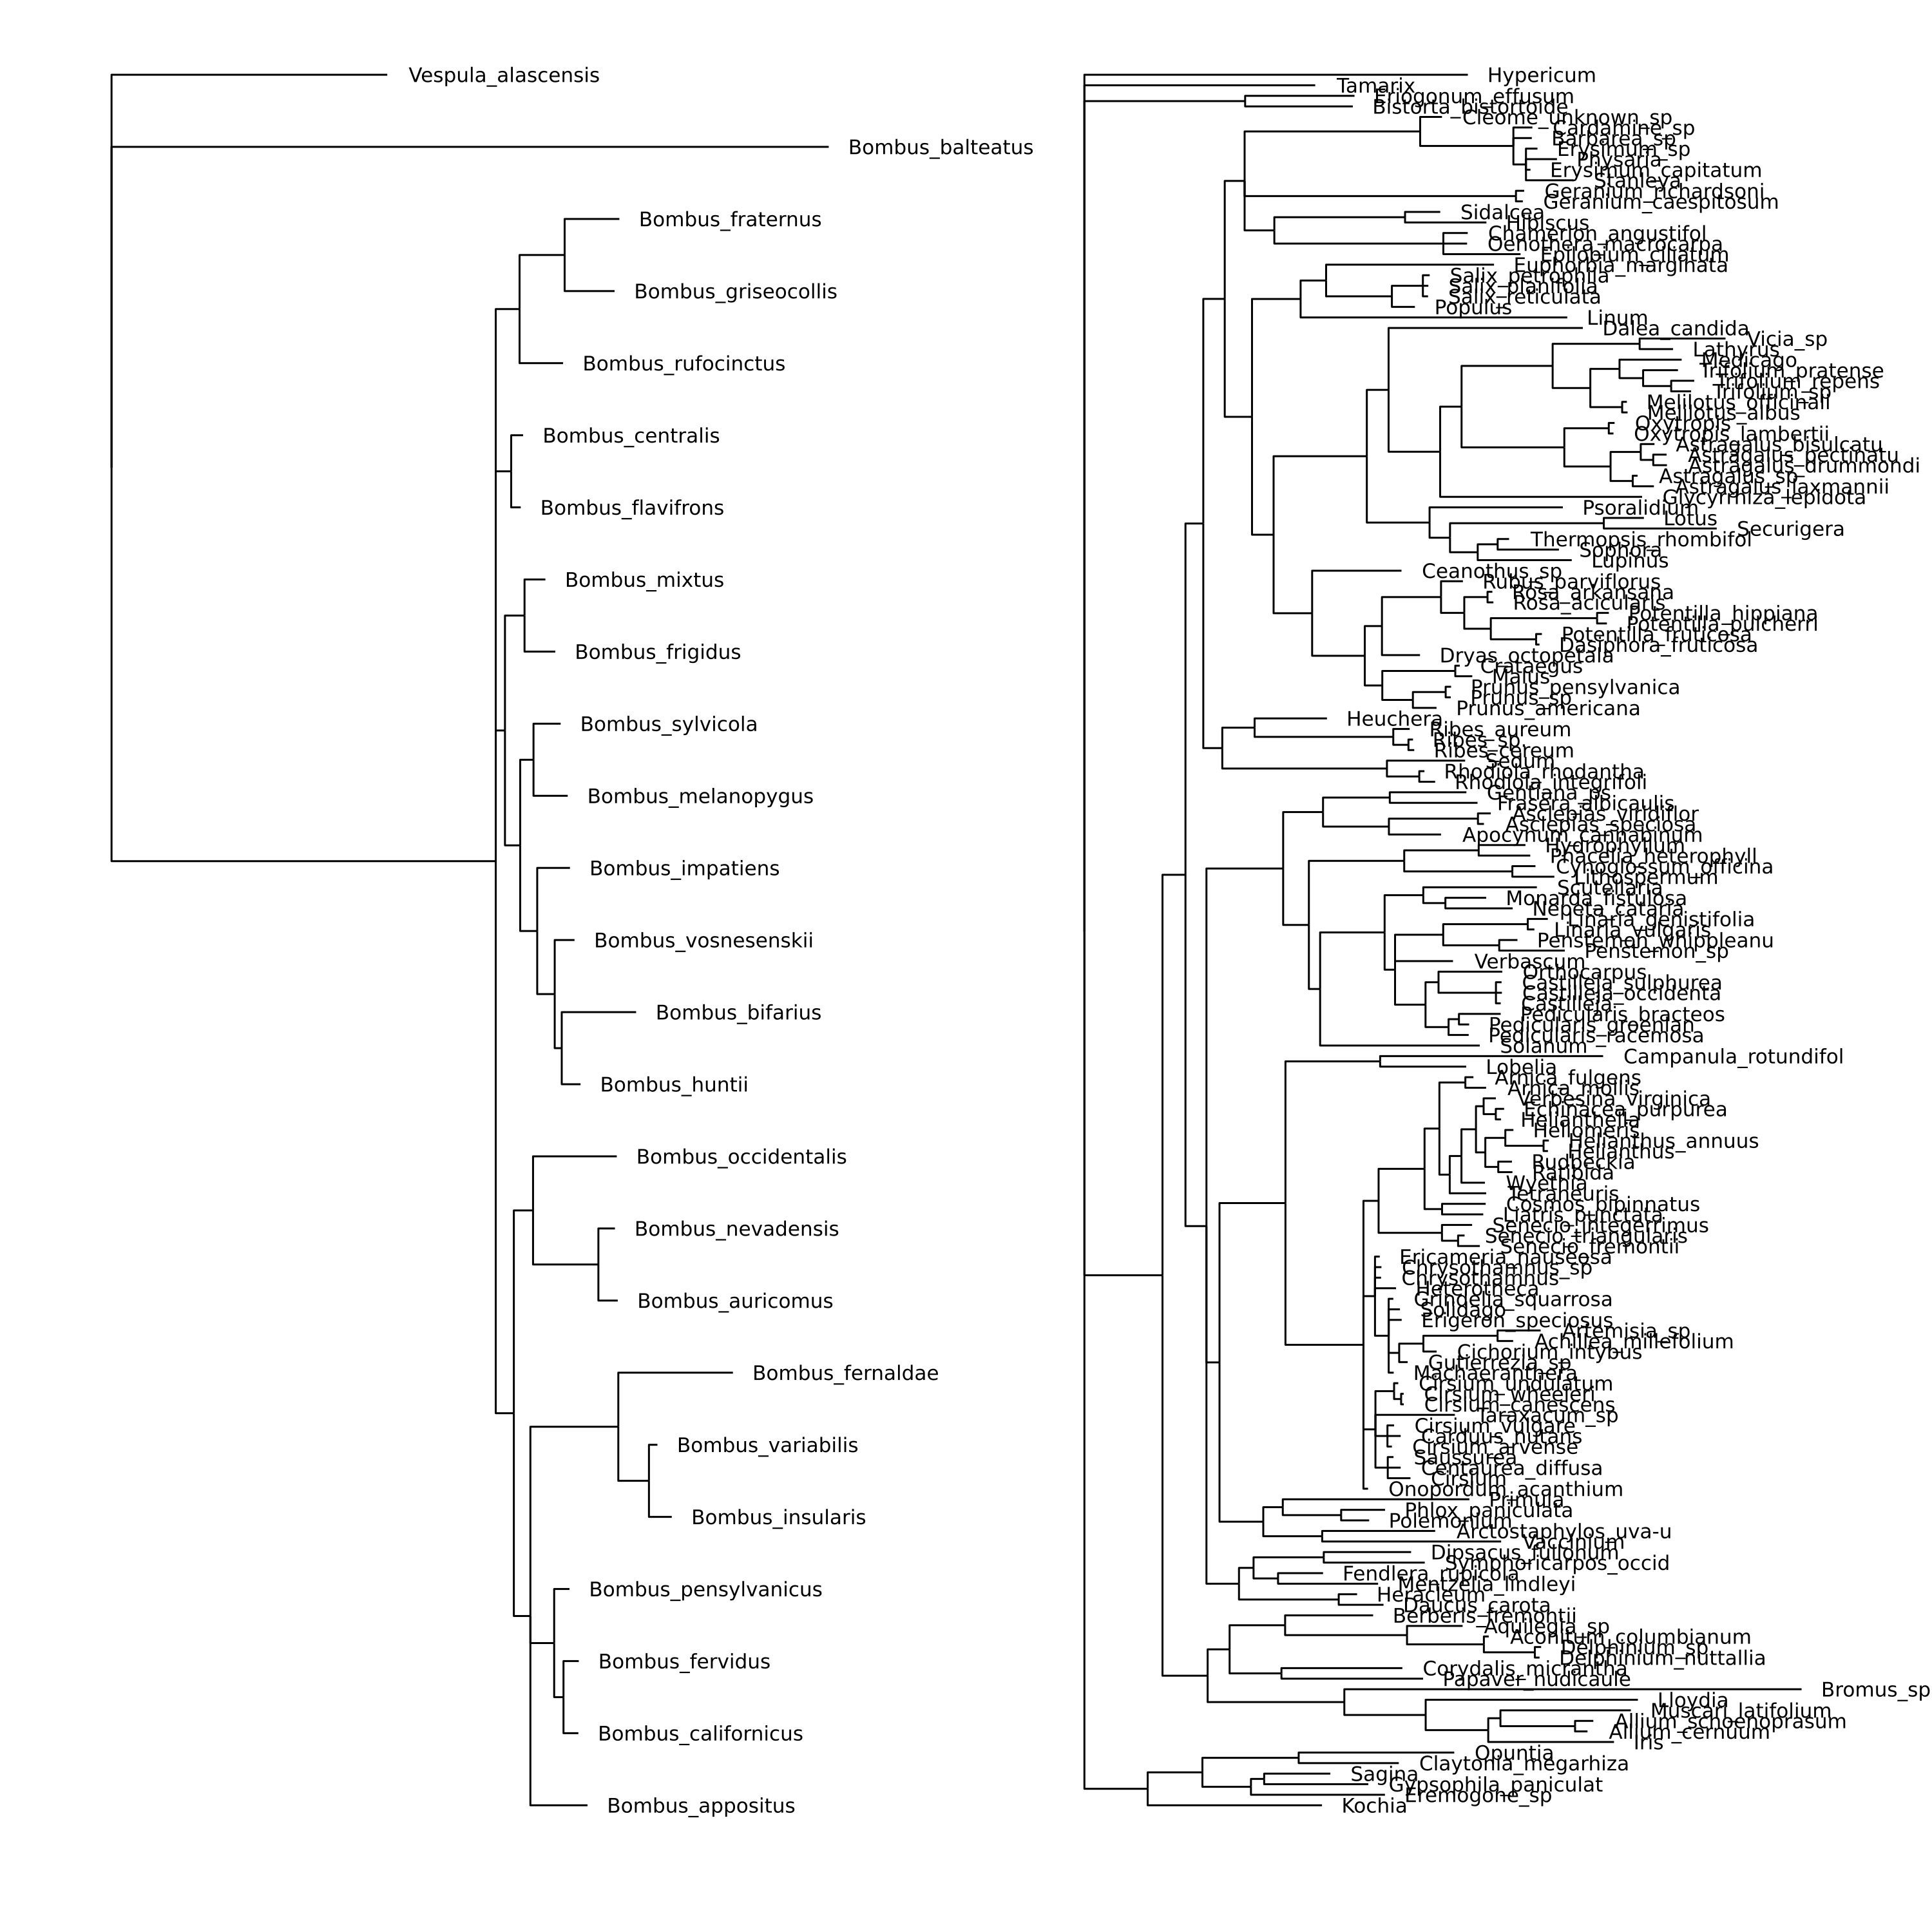
\includegraphics{./figures/trees.png}
\caption{trees}
\end{figure}

\hypertarget{references}{%
\section*{References}\label{references}}
\addcontentsline{toc}{section}{References}

\hypertarget{refs}{}
\begin{CSLReferences}{1}{0}
\leavevmode\hypertarget{ref-Bauer2015QuiRev}{}%
Bauer, P., Thorpe, A. \& Brunet, G. (2015). The quiet revolution of
numerical weather prediction. \emph{Nature}, 525, 47--56.

\leavevmode\hypertarget{ref-Beckage2011LimPre}{}%
Beckage, B., Gross, L.J. \& Kauffman, S. (2011). The limits to
prediction in ecological systems. \emph{Ecosphere}, 2, art125.

\leavevmode\hypertarget{ref-Blanchet2020CooNot}{}%
Blanchet, F.G., Cazelles, K. \& Gravel, D. (2020). Co-occurrence is not
evidence of ecological interactions. \emph{Ecology Letters}, 23,
1050--1063.

\leavevmode\hypertarget{ref-Chen2019RevCom}{}%
Chen, Y., Angulo, M.T. \& Liu, Y.-Y. (2019). Revealing Complex
Ecological Dynamics via Symbolic Regression. \emph{BioEssays}, 41,
1900069.

\leavevmode\hypertarget{ref-Dietze2017PreEco}{}%
Dietze, M.C. (2017). Prediction in ecology: A first-principles
framework. \emph{Ecological Applications}, 27, 2048--2060.

\leavevmode\hypertarget{ref-Hadfield2014TalTwo}{}%
Hadfield, J.D., Krasnov, B.R., Poulin, R. \& Nakagawa, S. (2014). A Tale
of Two Phylogenies: Comparative Analyses of Ecological Interactions.
\emph{The American Naturalist}, 183, 174--187.

\leavevmode\hypertarget{ref-Hanski2000MetCap}{}%
Hanski, I. \& Ovaskainen, O. (2000). The metapopulation capacity of a
fragmented landscape. \emph{Nature}, 404, 755--758.

\leavevmode\hypertarget{ref-Hill2004ArcEar}{}%
Hill, C., DeLuca, C., Balaji, Suarez, M. \& Da Silva, A. (2004). The
architecture of the Earth System Modeling Framework. \emph{Computing in
Science Engineering}, 6, 18--28.

\leavevmode\hypertarget{ref-Hubbell2001UniNeu}{}%
Hubbell, S.P. (2001). \emph{The unified neutral theory of biodiversity
and biogeography}. Monographs in population biology. Princeton
University Press, Princeton.

\leavevmode\hypertarget{ref-Levin1992ProPat}{}%
Levin, S.A. (1992). The Problem of Pattern and Scale in Ecology: The
Robert H. MacArthur Award Lecture. \emph{Ecology}, 73, 1943--1967.

\leavevmode\hypertarget{ref-Makiola2020KeyQue}{}%
Makiola, A., Compson, Z.G., Baird, D.J., Barnes, M.A., Boerlijst, S.P.,
Bouchez, A., \emph{et al.} (2020). Key Questions for Next-Generation
Biomonitoring. \emph{Frontiers in Environmental Science}, 7.

\leavevmode\hypertarget{ref-Ovaskainen2002MetMod}{}%
Ovaskainen, O., Sato, K., Bascompte, J. \& Hanski, I. (2002).
Metapopulation Models for Extinction Threshold in Spatially Correlated
Landscapes. \emph{Journal of Theoretical Biology}, 215, 95--108.

\leavevmode\hypertarget{ref-Ovaskainen2002MetMod}{}%
Ovaskainen, O., Sato, K., Bascompte, J. \& Hanski, I. (2002).
Metapopulation Models for Extinction Threshold in Spatially Correlated
Landscapes. \emph{Journal of Theoretical Biology}, 215, 95--108.

\leavevmode\hypertarget{ref-Pennekamp2019IntPre}{}%
Pennekamp, F., Iles, A.C., Garland, J., Brennan, G., Brose, U., Gaedke,
U., \emph{et al.} (2019). The intrinsic predictability of ecological
time series and its potential to guide forecasting. \emph{Ecological
Monographs}, 89, e01359.

\leavevmode\hypertarget{ref-Petchey2015EcoFor}{}%
Petchey, O.L., Pontarp, M., Massie, T.M., Kéfi, S., Ozgul, A.,
Weilenmann, M., \emph{et al.} (2015). The ecological forecast horizon,
and examples of its uses and determinants. \emph{Ecology Letters}, 18,
597--611.

\leavevmode\hypertarget{ref-Peterman2018ResRP}{}%
Peterman, W.E. (2018). ResistanceGA: An R package for the optimization
of resistance surfaces using genetic algorithms. \emph{Methods in
Ecology and Evolution}, 9, 1638--1647.

\leavevmode\hypertarget{ref-Strydom2021RoaPre}{}%
Strydom, T., Catchen, M.D., Banville, F., Caron, D., Dansereau, G.,
Desjardins-Proulx, P., \emph{et al.} (2021). \emph{A Roadmap Toward
Predicting Species Interaction Networks (Across Space and Time)}
(Preprint). EcoEvoRxiv.

\leavevmode\hypertarget{ref-Thompson2000ResSol}{}%
Thompson, R.M. \& Townsend, C.R. (2000). Is resolution the solution?:
The effect of taxonomic resolution on the calculated properties of three
stream food webs. \emph{Freshwater Biology}, 44, 413--422.

\leavevmode\hypertarget{ref-Urban2021CodLif}{}%
Urban, M.C., Travis, J.M.J., Zurell, D., Thompson, P.L., Synes, N.W.,
Scarpa, A., \emph{et al.} (2021). Coding for Life: Designing a Platform
for Projecting and Protecting Global Biodiversity. \emph{BioScience}.

\end{CSLReferences}

\end{document}
